\documentclass[tikz,border=4pt]{standalone}
\usepackage{amsmath,amssymb}
\usetikzlibrary{arrows.meta,decorations.pathmorphing}

\begin{document}
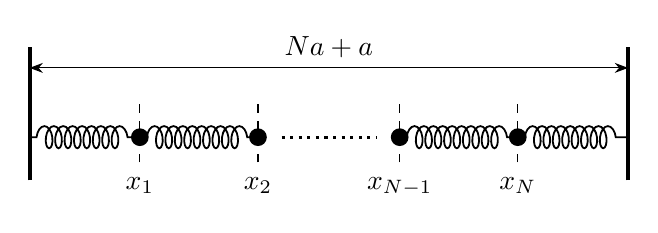
\begin{tikzpicture}[
  >=Stealth,
  font=\normalsize,
  axis/.style={line width=0.4pt},
  curve/.style={line width=0.9pt},
  spring/.style={line width=0.65pt,decorate,decoration={coil,amplitude=4pt,segment length=3.4pt,pre length=2.5pt,post length=2.5pt}}
]
  % Left and right walls
  \draw[line width=1.4pt] (0,-0.55) -- (0,1.15);
  \draw[line width=1.4pt] (7.6,-0.55) -- (7.6,1.15);

  % Total length Na + a
  \draw[axis,<->] (0,0.88) -- (7.6,0.88) node[midway,above] {$Na + a$};

  % Masses at x = 1.4, 2.9, 4.7, 6.2
  \draw[spring] (0,0) -- (1.4,0);
  \draw[spring] (1.4,0) -- (2.9,0);
  \draw[line width=1.1pt,dotted] (3.2,0) -- (4.4,0);
  \draw[spring] (4.7,0) -- (6.2,0);
  \draw[spring] (6.2,0) -- (7.6,0);

  \foreach \x/\lab in {1.4/x_1, 2.9/x_2, 4.7/x_{N-1}, 6.2/x_N} {
    \fill (\x,0) circle (3.2pt);
    \draw[axis,dashed] (\x,-0.32) -- (\x,0.45);
    \node[below=2pt] at (\x,-0.32) {$\lab$};
  }
\end{tikzpicture}
\end{document}
